\scanpage{301}

We denote by $S\Gamma^{!}_{g,\nu}$ and $S\unsure{\mathcal{E}|\varepsilon}^{!}_{g,\nu}$ the \unsure{subgroups|subgroups} of the preceding $S\Gamma_{g,\nu}$, $S\unsure{\mathcal{E}|\varepsilon}_{g,\nu}$ which induce the identity on $I=S_{g,\nu}$.

And let us finally return to the relations with $S\unsure{A|\mathcal A}_{g,\nu}$, we are going to define
\[
SA_{g,\nu}\longrightarrow S\Gamma^{!+}_{g,\nu}
\]
by \deleted{choosing for $\forall$} noting that if a $u\in A_{g,\nu}$ induces the identity in a neighborhood of $S_{g,\nu}$, then $\unsure{u_{\bullet}|u_i}(\unsure{\widetilde D_i^{*}|\widetilde D_i})\unsure{\simeq|=}\widetilde D_i^{*}$ and we shall be able to define an element of $S\Gamma^{!}_{g,\nu}$ by taking as $\gamma_i$ the identities. The fact that the homomorphism obtained is trivial on $(SA_{g,\nu})^0$ is probably trivial, hence
\[
SA_{g,\nu}/(SA_{g,\nu})^0\longrightarrow S\Gamma^{!+}_{g,\nu}.
\]
To say that this is surjective means that $\forall$ automorphism $\in A_{g,\nu}^{!+}$ \inserted{(i.e. \unsure{all|the} automorphisms of $U_{g,\nu}$ inducing the identity on $S_{g,\nu}$ and respecting the orientation)} is isotopic (by an isotopy, \unsure{if one wishes}, which remains the identity outside a small neighborhood of $S_{g,\nu}$) to an automorphism which is the identity on a neighborhood, this is easy. Injectivity perhaps more delicate, it comes down essen

\mspage{300}

\scanpage{302}
\mspage{152}

tially to: determining the kernel of
\[
S\unsure{A|\mathcal A}_{g,\nu}/(SA_{g,\nu})^0\longrightarrow\Gamma^!_{g,\nu},
\quad\text{i.e.}\quad
SA_{g,\nu}\cap A_{g,\nu}^0/(SA_{g,\nu})^0
\]
as $T^I=T^{S_{g,\nu}}$. We can probably reduce to the context of \inserted{compact} surfaces with boundary (let us denote by a $'$ the corresponding topological groups), we have
\[
1\longrightarrow SA_{g,\nu}^{\prime+}\longrightarrow
A_{g,\nu}^{\prime!+}\longrightarrow
\prod_{i\in S_{g,\nu}}\operatorname{Aut}^+(C_i)\longrightarrow1
\]
\margin{homotopic to the standard \unsure{circle} \deleted{\illegible{1}} group $\mathbb U$, twisted by $\unsure{T|\Pi}$}
where the $+$ indicates the automorphisms preserving the \unsure{orientation}, and the $C_i$ are the connected components of the boundary. We conclude from this the homotopy exact sequence
\LMlayoutnotice{140-2-302-D1}
\begin{landscape}
\begin{center}
\begin{tikzcd}[ampersand replacement=\&,column sep=small,row sep=small,column sep=9pt,row sep=14pt,execute at begin picture={\fontsize{10}{12}\selectfont}]
\inserted{0=\unsure{\prod_i|\prod}\unsure{\Pi_2|\pi_2}(\operatorname{Aut}^+(C_i))}
\arrow[r] \&
\unsure{\Pi_1|\pi_1}(SA_{g,\nu}^{\prime0})\arrow[r] \&
\unsure{\Pi_1|\pi_1}(A_{g,\nu}^{\prime!+})\arrow[r]\arrow[d,equal] \&
\deleted{\unsure{\Pi_0}}\prod_i\unsure{\Pi_1|\pi_1}(\operatorname{Aut}^+(C_i))\arrow[r]\arrow[d,phantom,"\unsure{\wr}"] \&
\unsure{\Pi_0|\pi_0}(SA_{g,\nu}^{\prime+})\arrow[r] \&
\unsure{\Pi_0|\pi_0}(A_{g,\nu}^{\prime!+})\arrow[d,equal]\arrow[dd,bend left=28] \\
\&\&\unsure{\Pi_1|\pi_1}(A_{g,\nu}^{\prime0})\&\unsure{T^I}\&\overset{\uparrow}{\uline{\text{to be computed}}}\&\Gamma_{g,\nu}'\\
\&\&\&\&\&1=\prod_i\unsure{\Pi_0|\pi_0}(\operatorname{Aut}^+(C_i))
\end{tikzcd}\end{center}
\end{landscape}
\[
\left[\text{and}\quad
\unsure{\Pi_i|\pi_i}(SA'_{g,\nu})\xrightarrow{\sim}
\unsure{\Pi_i|\pi_i}(A_{g,\nu}^{\prime\unsure{0}})
\quad\text{if }i\geq2\right]
\]

i.e.
\[
\left\{\begin{aligned}
0&\longrightarrow\unsure{\Pi_1|\pi_1}(SA_{g,\nu}^{\prime+})
\longrightarrow\unsure{\Pi_1|\pi_1}(A_{g,\nu}^{\prime0})
\longrightarrow T^I\longrightarrow\unsure{\Pi_0|\pi_0}(SA_{g,\nu}^{\prime!+})
\longrightarrow\Gamma_{g,\nu}^{\prime!+}\longrightarrow1.\\
&\unsure{\Pi_i|\pi_i}(SA_{g,\nu}^{\prime+})\xrightarrow{\sim}
\deleted{\illegible{1}}\unsure{\Pi_i|\pi_i}(A_{g,\nu}^{\prime0})
\quad\text{for }i\geq2
\end{aligned}\right.
\]
\deleted{In the case \illegible{1}}

We have an obvious homomorphism: (by '\unsure{gluing} disks')
$A_{g,\nu}^{\prime\unsure{0}}\longrightarrow A_{g,\nu}$ inducing
$SA'_{g,\nu}\longrightarrow SA_{g,\nu}$,
\deleted{which} and these are surely homotopy equivalences, so
\deleted{\illegible{1}} the preceding exact sequence

\mspage{301}

\scanpage{303}

must be interpretable as an exact sequence
\[
\left\{\begin{aligned}
0&\longrightarrow\unsure{\Pi_1|\pi_1}((S\unsure{A|\mathcal A}_{g,\nu})^0)
\longrightarrow\unsure{\Pi_1|\pi_1}(A_{g,\nu}^0)
\longrightarrow T^I\longrightarrow\unsure{\Pi_0|\pi_0}(SA_{g,\nu}^{!+})
\longrightarrow\unsure{\Gamma}_{g,\nu}^{!+}\longrightarrow1\\
&\unsure{\Pi_i|\pi_i}((SA_{g,\nu})^0)\xrightarrow{\sim}
\unsure{\Pi_i|\pi_i}(A_{g,\nu}^0)\quad\text{for }i\geq2.
\end{aligned}\right.
\]

In the anabelian case, we do indeed find, \unsure{since}
$\unsure{\Pi_1|\pi_1}(A_{g,\nu}^0)=0$, an extension structure
\[
\boxed{1\longrightarrow T^{S_{g,\nu}}\longrightarrow
\unsure{\Pi_0|\pi_0}(SA_{g,\nu})\longrightarrow\Gamma_{g,\nu}^{!+}\longrightarrow1}
\]
\deleted{\unsure{from which we deduce} $1\longrightarrow T^{S_{g,\nu}}\longrightarrow\unsure{\Pi_0|\pi_0}(\unsure{S}$}
and moreover
\[
\unsure{\Pi_i|\pi_i}((SA_{g,\nu})^0)=0\quad\text{for }i\geq2.
\]

In the abelian case, we must make explicit
\deleted{\illegible{1}}
\[
\unsure{\Pi_1|\pi_1}(A_{g,\nu}^0)\longrightarrow T^{S_{g,\nu}}
\]
and we are going to distinguish the \deleted{four}\inserted{two} abelian cases
\inserted{(\unsure{with the understanding} that we have $I\ne\varnothing$!) --- \unsure{we have|i.e.} always $g=0$, $\nu=1$ or $2$. \deleted{\unsure{As}}}

In any case, introducing a \unsure{complex|complex} analytic structure and the group $G$, identity component of the group of complex automorphisms, we have
\unsure{have}
\[
G\xrightarrow{\unsure{\approx|\sim}}A_{g,\nu}^0.
\]
\deleted{\unsure{thus}} :

a) Case $g=0$, $\nu=2$ \deleted{\unsure{thus} $I\unsure{=|\ne}\varnothing$}
$G\simeq\mathbb C^*$, \deleted{it operates}
we see that if the loop structure \inserted{of $\unsure{\pi|\Pi}$} is defined by the two isomorphisms
$\unsure{k_i|\kappa_i}:T\longrightarrow\unsure{\pi|\Pi}$
$(i\in I=\{\unsure{s_{g0}|s_{0,0}|s_\infty},\unsure{s_{0g}|s_{0,1}|s_0}\})$

\mspage{302}

\scanpage{304}
\mspage{153}

then $\unsure{\Pi_1|\pi_1}(G)\longrightarrow T^I$ is identified with
$T\longrightarrow T^I$ whose components are \unsure{these|the} two
$\unsure{k_i|\kappa_i}$ (which are symmetric, so this is an injective homomorphism whose image is the kernel of the sum map
$T^I\longrightarrow T$, so \unsure{here} the kernel of
\diagram{\begin{tikzcd}[ampersand replacement=\&,column sep=small,row sep=small]
\unsure{\Pi_0|\pi_0}(S\unsure{A|\mathcal A}_{g,\nu})\arrow[r]\&\Gamma_{g,\nu}^{!+}\arrow[d,equal]\\
\&\unsure{0}\deleted{\unsure{\text{zero}}}
\end{tikzcd}}
(\unsure{of which|thus} $\unsure{\Pi_0|\pi_0}(SA_{g,\nu})$ itself)
\unsure{is} isomorphic, not to $T^I$, but to its quotient $T$.
As for $(SA'_{g,\nu})^0$, all its $\unsure{\Pi_i|\pi_i}$ $(i\geq1)$ are zero --- it is again $\infty$-connected.

b) Case $g=0$, $\nu=1$. Then $G\simeq\unsure{\operatorname{Aff}(1,\mathbb C)}$,
$\unsure{\Pi_1|\pi_1}(G)\simeq T$ and
$\unsure{\Pi_1|\pi_1}(G)\longrightarrow T^I=T$ is an isomorphism.
Here, \deleted{\unsure{again}} the kernel of the homomorphism
\diagram{\begin{tikzcd}[ampersand replacement=\&,column sep=small,row sep=small]
\unsure{\Pi_0|\pi_0}(SA_{g,\nu})\arrow[r]\&\Gamma_{g,\nu}^{!+}\arrow[d,phantom,"\unsure{\wr}"]\\
\&\unsure{0}
\end{tikzcd}}
is zero
\deleted{(\unsure{formally|formally}, it would be defined as \illegible{1} in the preceding case)}
\figure{[V-shaped mark to the right of this 0, at the end of the first struck-out line.]}
i.e. \deleted{it is an isomorphism} $\unsure{\Pi_0|\pi_0}(SA_{g,\nu})=0$.
In this case too, we find that $\unsure{\Pi_i|\pi_i}(SA_{g,\nu}^0)=0$
for \unsure{every} $i\geq\unsure{1}$. We therefore find

\uline{Theorem} \inserted{Suppose $\nu\unsure{>|\geq}0$.}
If $(g,\nu)$ is anabelian, then $\unsure{\Pi_0|\pi_0}(SA_{g,\nu})$ is canonically isomorphic to $S\Gamma_{g,\nu}^{!+}$.
In all cases, $(SA_{g,\nu})^0$ is $\infty$-connected.
\figure{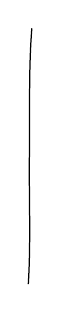
\begin{tikzpicture}[x=1cm,y=1cm]
\draw[line width=0.45pt] (0.045,3.25)
  .. controls (0.005,2.76) and (0.020,2.23) .. (0.015,1.70)
  .. controls (0.005,1.18) and (0.035,0.57) .. (0,0);
\end{tikzpicture}}

\mspage{303}

\scanpage{305}
We are going to make explicit a compatibility
relation for $S\Gamma$ relative to a $\pi$
with \unsure{loops}, fixing an $i\in I=\unsure{\mathcal I(\pi)}$,
hence a stabilizer $\Gamma_i\subset\Gamma$ whose inverse
image $(S\Gamma)_i$ in $S\Gamma$ is thus an
extension of $\Gamma_i$ by $T^I$. Using the
projection $T^I\xrightarrow{\mathrm{pr}_i}T$, we find an
extension of $\Gamma_i$ by $T$, which we are going to describe
in another way. The extension $S\Gamma$
is defined intrinsically by the
datum of $I$ \unsure{realizations} \inserted{$(\pi_i)_{i\in I}$} \unsure{of the group}
\unsure{outer} $\pi$ by groups, with in
each $\pi_i$ an $L_i\subset\pi_i$ of class $i$
(that is it, the datum of a system of the
$(\widetilde D_i^*)$!). For an outer automorphism \deleted{\unsure{$u$}} \inserted{with loops $u\in\Gamma$} of $\pi$,
\deleted{its ``\illegible{1}'' are the}
for $\forall i$ it \deleted{\unsure{there are ways}} \inserted{is possible} to
\unsure{realize} it by $u_i\in\operatorname{Aut}_{\unsure{\mathrm{lac}|\mathrm{loc}}}(\pi_i)$, with $u_i(L_i)\subset L_i$
--- this $u_i$ is determined \unsure{modulo} right
multiplication by an $\operatorname{int}(\unsure{k_i|\kappa_i}(\alpha))$, where $\alpha\in T$.
Of course, $S\Gamma$ is the \unsure{subgroup} \unsure{of the|of the}
\mspage{304}

\scanpage{306}
\mspage{154}
$\displaystyle\prod_{i\in I}\operatorname{Aut}_{\unsure{\mathrm{lac}|\mathrm{loc}}}(\pi_i)$,
\deleted{\unsure{formed of} \illegible{1}} \inserted{\unsure{the inverse image}} of the diagonal
under the natural homomorphism from this product to
$\operatorname{Autext}_{\unsure{\mathrm{lac}|\mathrm{loc}}}(\pi)^I$, \deleted{\unsure{whence an}} \inserted{\unsure{which is indeed}} extension of
\unsure{the said} diagonal (identified with $\Gamma$) by $T^I$.
If we look at the subextension \deleted{of $\Gamma_i$} obtained
by restriction to $\Gamma_i$, we see that the
projection $T^I\unsure{\xrightarrow{\mathrm{pr}_i}}T$ is stable under $\Gamma_i$; thus
we deduce from it an extension of $\Gamma_i$ by $T$,
which is none other than the group of
automorphisms \inserted{with loops} of $\pi_i$ which normalize $L_i$
--- which is indeed an extension of $\Gamma_i$ by $L_i$
(\unsure{for} intersection with $\pi_i\subset\operatorname{Aut}_{\unsure{\mathrm{lac}|\mathrm{loc}}}(\pi_i)$ \unsure{is|being}
reduced to $L_i$).

This shows us that the extension
of $\Gamma$ by $T^I$ has a marked tendency
not to be trivial, for this is \unsure{so}
\inserted{(for $i\in I$ fixed)} for the extension of $\Gamma_i$ by $T$ \inserted{to} which it gives
rise. If for example we have a
\uline{finite} subgroup $G\subset\Gamma_i^+$, the induced extension is
never trivial if $G\ne1$, we have seen this. In
fact, $G$ must be cyclic and its inverse image
in the extension in question is $\simeq T$\ldots
\mspage{305}

\scanpage{307}
\mspage{155}
$25^{\mathrm{bis}}$. Case of the two groups. Return to the \unsure{notations}

We place ourselves \inserted{first} to fix ideas in the
topological and discrete case, but the motivation is
the case of an algebraic curve $U$ over a
finitely generated field $K$, where we have both
the group $G_K=\operatorname{Aut}_K(U)$ and $\Gamma=\operatorname{Gal}(\overline K/K)$
\margin{Anabelian case so \unsure{$G$|$G_K$} finite}
which \unsure{operate} by outer automorphisms on $\pi_1(U_{\overline K})$.
In this case, $G$ and $\Gamma$ commute, but
we can look more generally at the case
of the group (bigger than $G_K$) $G_{\overline K}=\operatorname{Aut}_{\overline K}(U)$,
on which $\Gamma$ operates (in a not necessarily trivial way
--- this operation describes \unsure{a} finite étale
algebraic group over $K$.

So suppose we have a surface
$U$ (orientable, $U=X-S$, $X$ \unsure{compact} \inserted{\unsure{connected}}, $S$ finite)
on \unsure{which|which} \unsure{operate} two groups $G$, $\Gamma$,
the action of $\Gamma$ normalizing that of $G$
--- so we have a group $\mathcal G=\Gamma . G$ (semidirect
product, for a certain action of $\Gamma$
on $G$) which operates on $U$. We suppose $G$
finite, but not necessarily $\Gamma$ finite.
\mspage{306}

\scanpage{308}

We suppose chosen a universal covering $\widetilde U$ of $U$, hence a group with \unsure{loops} $\pi=\operatorname{Aut}(\widetilde U)$, on which $\mathcal G$ operates by outer automorphisms, hence extension
\[
(1)\qquad 1\longrightarrow\pi\longrightarrow\unsure{\mathcal E|\varepsilon}\longrightarrow\mathcal G\longrightarrow 1
\]
\margin{We are going to \unsure{suppose} the action of $\mathcal G$ faithful}
If the action of $\mathcal G$ on $U$ \inserted{modulo isotopy} is faithful,
then $\mathcal G\hookrightarrow\operatorname{Autext}(\pi)$, and the preceding extension is the inverse image of the Teichmüller extension of $\pi$
\[
1\longrightarrow\pi\longrightarrow\operatorname{Aut}_{\mathrm{lac}}(\pi)\longrightarrow\operatorname{Autext}_{\mathrm{lac}}(\pi)\longrightarrow 1.
\]

\deleted{\unsure{Let}} We shall have to look at other universal \unsure{covering\textsuperscript{s}} than $\widetilde U$, and their isomorphisms with $\widetilde U$.
When $\widetilde U=\widetilde U(P)$ is the universal covering based at a certain $P\in U$, then for universal coverings \inserted{$\unsure{U(Q)}$} based at \deleted{\illegible{1}} \inserted{a} \unsure{point\deleted{s}|points},
the \inserted{$U$-}isomorphisms $\widetilde U(P)\xrightarrow{\sim}\unsure{\overline U(Q)|\widetilde U(Q)}$ correspond \unsure{thus} to the classes of paths from $P$ to $Q$.

Let \deleted{\illegible{1}} $Q\in U$ be such that its isotropy group \inserted{$G_Q$} \deleted{\illegible{1}} \uline{in $G$} is \unsure{such} that $G_Q^+\ne1$.
(So $G_Q^+$ is cyclic). Choosing a
\mspage{307}

\scanpage{309}
\mspage{156}

class of paths \inserted{$\lambda$} from $P$ to $Q$, identifying $\unsure{\overline U(P)|\widetilde U(P)}$ with $\unsure{\overline U(Q)|\widetilde U(Q)}$, we find an operation of $G_Q$ on $\widetilde U(P)$ i.e. a lifting $G_Q\xrightarrow{r_{G_Q}}\unsure{\mathcal E|\varepsilon}$ in the extension (1) --- the change of class of paths \inserted{from $\lambda$ to $\lambda'$} will give a lifting $r'_{G_Q}$ which \deleted{\unsure{is}} will be conjugate to $r$ by a unique element of $\pi$ \inserted{$=\pi_1(U,P)$} (uniqueness comes from $\pi^{G_Q}=\{1\}$), \unsure{namely} the one which makes one \unsure{pass} from one path to another.

Let us consider the stabilizer $\Gamma_Q$ of $Q$ in $\Gamma$, \deleted{\illegible{2}} which of course operates on $\widetilde U(Q)$ just like $G_Q$ (in fact it is $\mathcal G_Q$ which operates \inserted{hence $r:\mathcal G_Q\to\unsure{\mathcal E|\varepsilon}$} \unsure{\dots}), so via $\lambda$ we also have a \unsure{lift\textsuperscript{ing}|lifting} $r_{\Gamma_Q}:\Gamma_Q\longrightarrow\unsure{\mathcal E|\varepsilon}$, which \inserted{has} even the \unsure{property} of \unsure{normalizing} $r_{G_Q}$ (\unsure{i.e.} operation of \deleted{\illegible{1}} $\Gamma_Q$ on it, which is the one coming from the given operation of $\Gamma$ on $G$).
\margin{\uline{N.B.} As the set \deleted{\illegible{1}} \unsure{of} points $Q$ is finite, and $\mathcal G$ operates on it, the orbit of $Q$ under $\mathcal G$ is finite, i.e. $\mathcal G_Q$ of finite index in $\mathcal G$. and likewise $\Gamma_Q$ in $\Gamma$.}
To simplify, let us suppose all the same that $\Gamma$ operates \unsure{trivial\textsuperscript{ly}} on $G$ i.e. $\mathcal G=\Gamma\times G$, then $r_{\Gamma_Q}(\Gamma_Q)\subset\unsure{\mathcal E|\varepsilon}$ is contained in the \uline{centralizer} of \inserted{$r$ (or of} $\unsure{r_{G_Q}}(G_Q)$),
\mspage{308}

\scanpage{310}

and since $\pi^{r(G_Q)}=1$, so the homomorphism
\[
\operatorname{Centr}(r_{\deleted{\unsure{G_Q}}}(G_Q))\longrightarrow\mathcal G
\]
is injective, the lifting in question \inserted{$\unsure{r_{\Gamma_Q}}$} is uniquely determined by the preceding condition.
\margin{\uline{N.B.} \unsure{Independent\textsuperscript{ly}|Independently} of \unsure{every|the} hypothesis that $\Gamma$ centralizes $G$, the normalizer of $r(G_Q)$ in $\pi$, equal to its ``centralizer'', is reduced to $1$, so $\operatorname{Norm}(r(G_Q))\longrightarrow\mathcal G$ is injective}

In fact, the image of $\operatorname{Centr}(r(G_Q))$ in $\mathcal G$ contains $\mathcal G_Q$, \inserted{\unsure{and}} \deleted{\illegible{5}} \unsure{even} the lifting $\mathcal G_Q\xrightarrow{r_{\mathcal G_Q}}\unsure{\mathcal E|\varepsilon}$.
\deleted{if $\mathcal G$ is finite}
\unsure{The|The} \unsure{interesting} thing is that \unsure{the|the} \inserted{choice of a} lifting\deleted{\unsure{s}} \unsure{of the|of the} (small) group $G_Q$, already imposes the choice of a lifting \unsure{of the|of the} (big) group $\Gamma_Q$, or $\mathcal G_Q$.

\deleted{When $\mathcal G$ is itself finite,} I say that the image in $\mathcal G$ of the centralizer \inserted{(and even of the normalizer)} of $r(G_Q)$ is $\mathcal G_Q$ itself (a priori it contains it).
\unsure{Returning|Let us return} to $\widetilde U(Q)$ itself, this means that \deleted{\illegible{1}} if $g\in\mathcal G$ is such that there exists an automorphism $\widetilde g$ of $\widetilde U(Q)$ which lifts $g$, while \deleted{\unsure{commuting}} \inserted{normalizing} \deleted{\unsure{with}} \inserted{the action of} $G_Q$, then $g\in\mathcal G_Q$ \inserted{(and $\widetilde g$ is the obvious lifting)}. Indeed, if $\widetilde g$ \deleted{\unsure{commutes}} \inserted{normalizes} \inserted{the action of} $G_Q$, it \unsure{leaves invariant|sends} the set of fixed points of $G_Q$ in $\widetilde U(Q)$, which is reduced \deleted{\illegible{1}} \inserted{\unsure{to the point}} $\unsure{\widetilde Q|\overline Q}$
\mspage{309}
